\documentclass[a4paper,12pt]{article}
\usepackage[margin=1in]{geometry}
\usepackage{booktabs}
\usepackage{graphicx}
\usepackage{float}

\begin{document}

\title{Additional Experimental Analysis: Lung Histopathological Image Classification}
\author{Experimental Results Report}
\date{\today}
\maketitle

\section{Additional Evaluation Metrics}
The following table reports the extended evaluation metrics for the best performing model (Grouping 3 with $\tau = 0.9$ and DenseNet121+SE backbone).

\begin{table}[H]
\centering
\caption{Detailed metrics for the best performing grouping operator (GP3, $\tau=0.9$)}
\begin{tabular}{lc}
\toprule
\textbf{Metric} & \textbf{Value} \\
\midrule
Accuracy & 0.9970 \\
Sensitivity (Recall) & 0.9970 \\
Specificity & 0.9985 \\
F1-Score & 0.9970 \\
AUC (ROC) & 1.0000 \\
MCC & 0.9955 \\
\bottomrule
\end{tabular}
\end{table}

\section{Attention Module Comparison}
We evaluated various attention mechanisms integrated with the DenseNet121 backbone. The Vision Transformer (ViT) and Swin Transformer modules performed the best in our experiments.

\begin{table}[H]
\centering
\caption{Comparison of different attention mechanisms}
\begin{tabular}{lcccc}
\toprule
\textbf{Attention Module} & \textbf{Accuracy} & \textbf{F1-Score} & \textbf{Features} & \textbf{Attn. Params} \\
\midrule
SE & 0.9970 & 0.9970 & 510 & 132,160 \\
ECA & 0.9967 & 0.9967 & 494 & 3 \\
CBAM & 0.9367 & 0.9362 & 538 & 132,259 \\
SPLIT & 0.9907 & 0.9907 & 519 & 83,008 \\
DUAL & 0.9973 & 0.9973 & 504 & 1,185,856 \\
\textbf{ViT} & \textbf{0.9983} & \textbf{0.9983} & 516 & 4,200,448 \\
\textbf{Swin} & \textbf{0.9983} & \textbf{0.9983} & 516 & 4,200,448 \\
\bottomrule
\end{tabular}
\end{table}

\section{Detailed Analysis Plots}
The following plots illustrate the sensitivity of the classification accuracy to various hyper-parameters, maintaining $\tau = 0.9$ as fixed.

\begin{figure}[H]
\centering
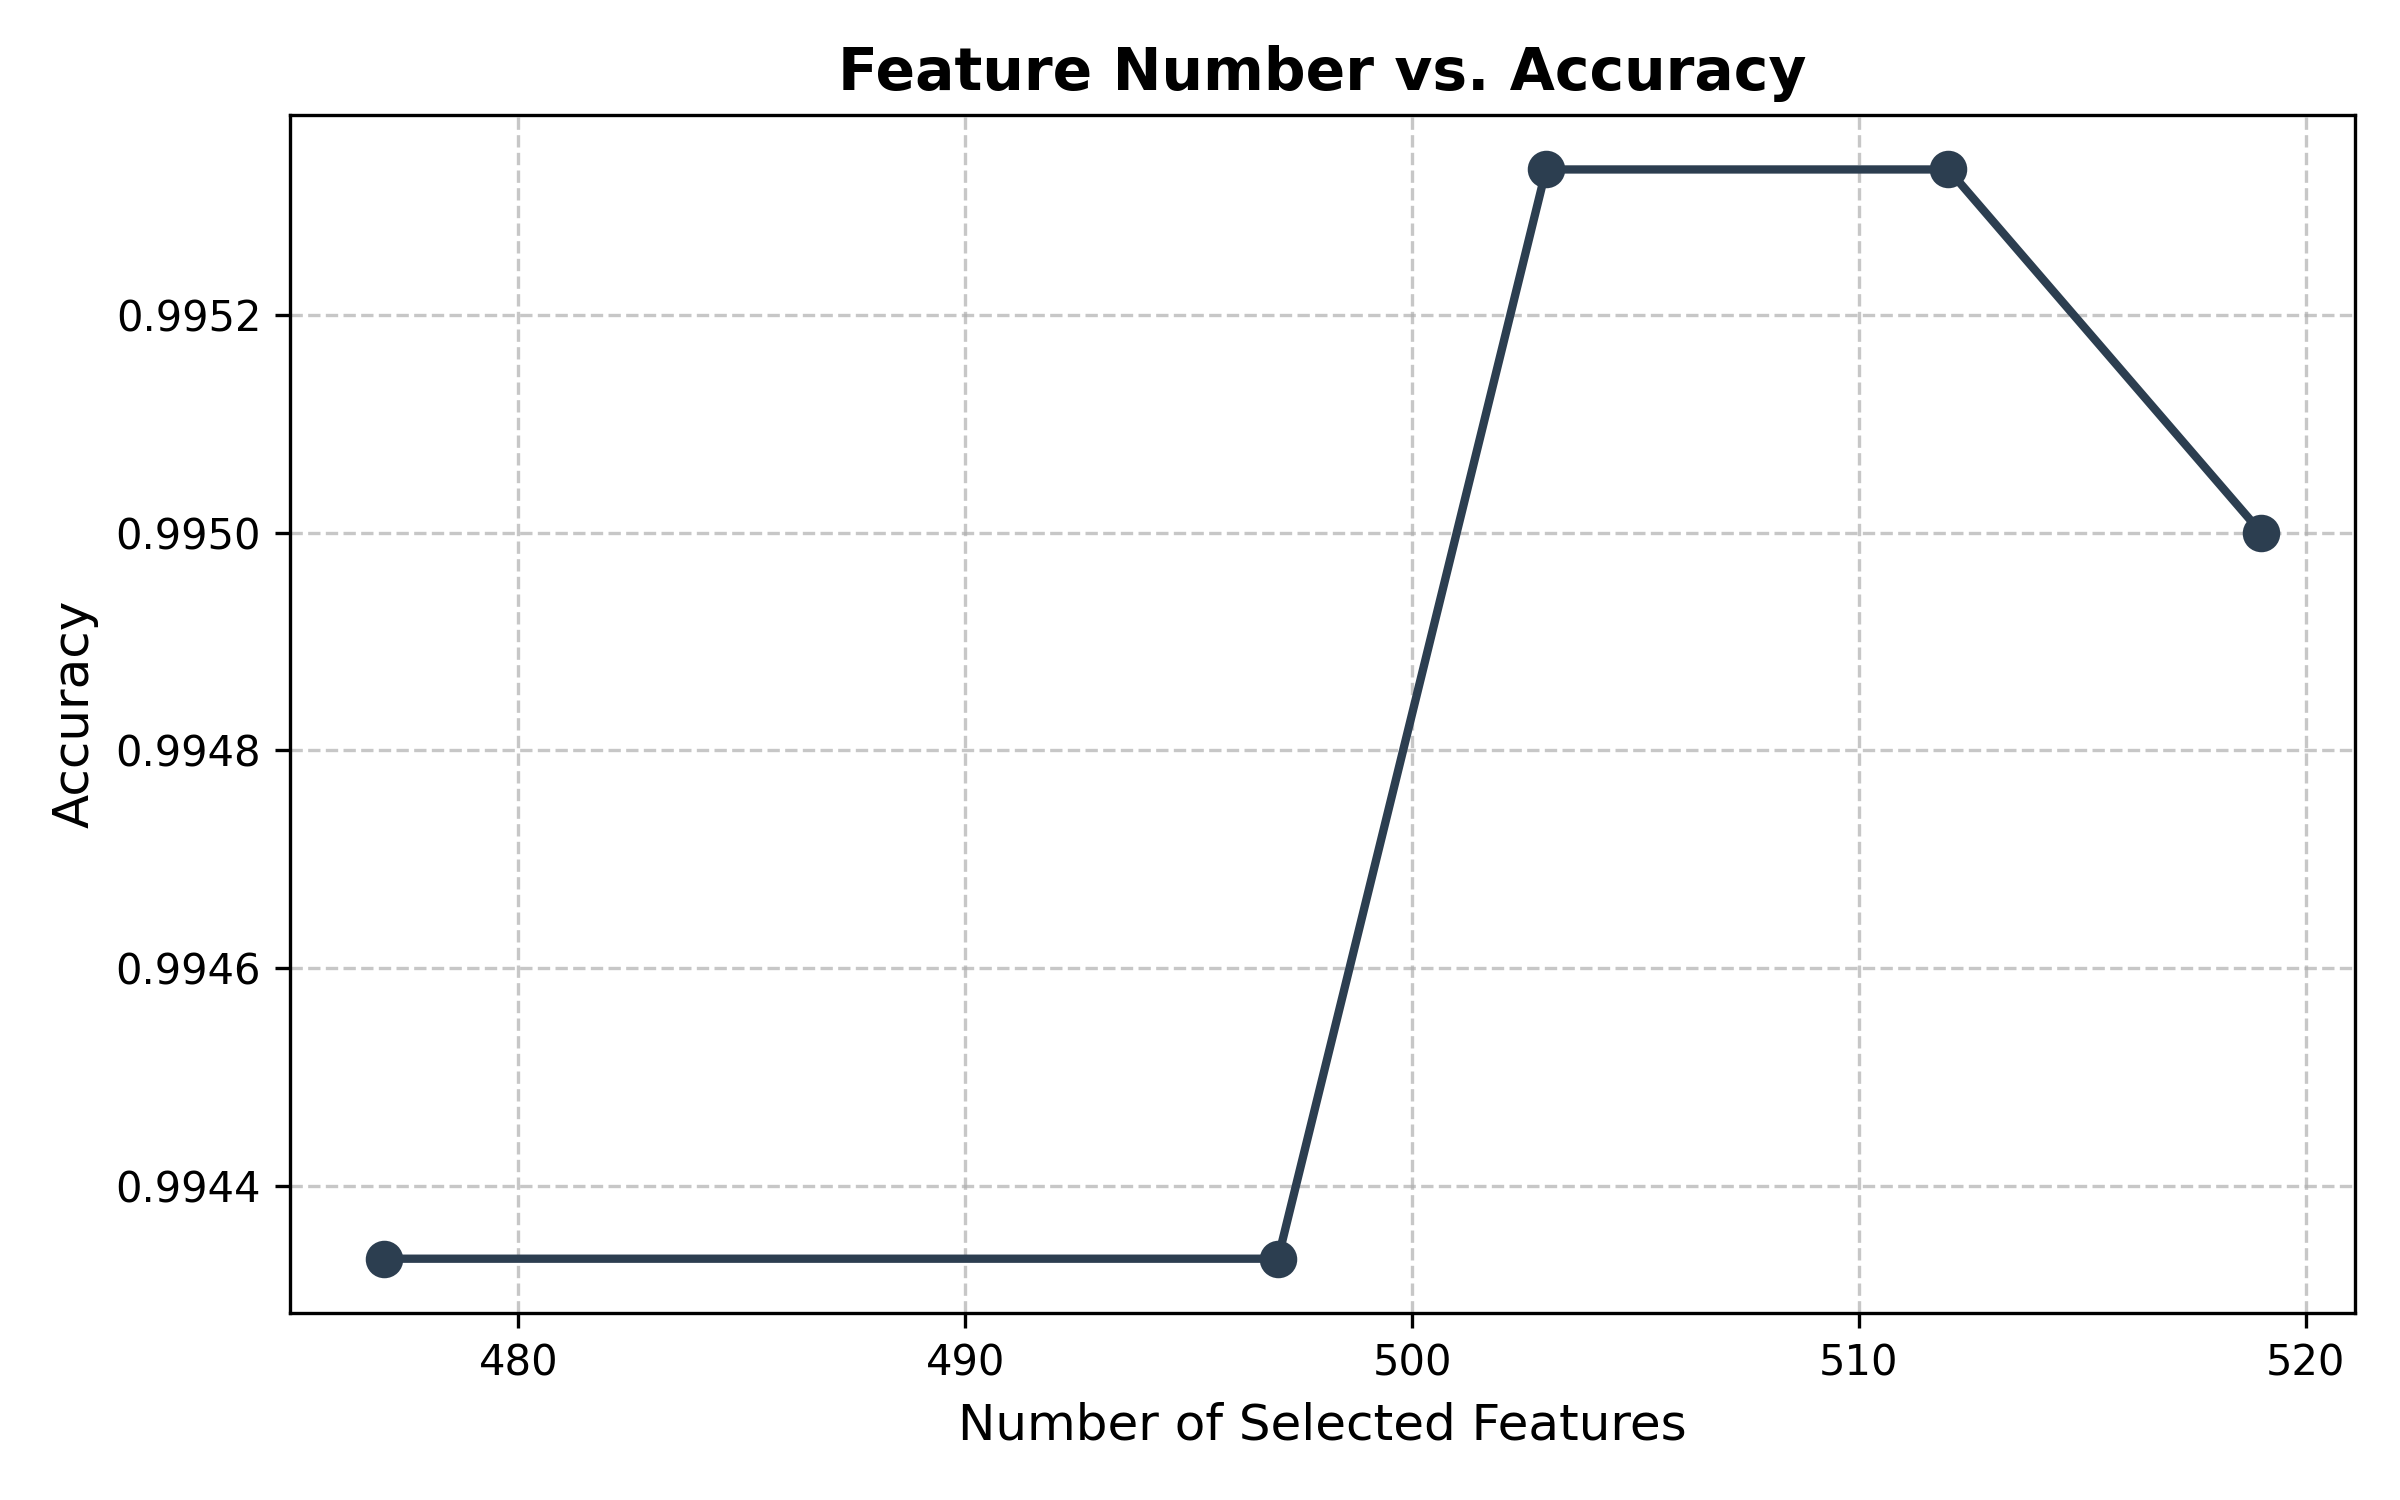
\includegraphics[width=0.48\textwidth]{figures/prof_feat_vs_acc.png}
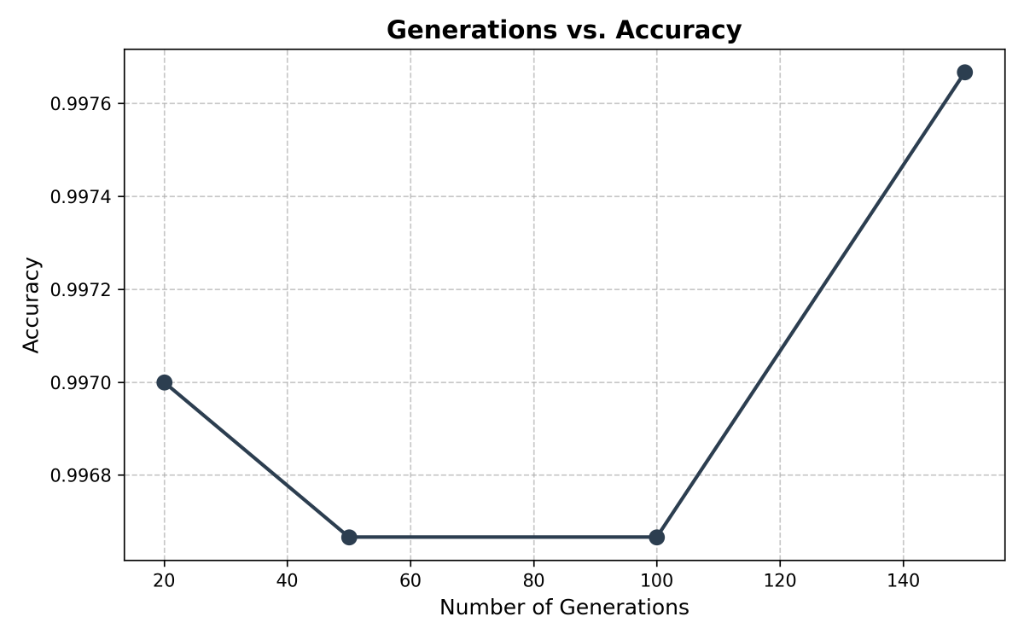
\includegraphics[width=0.48\textwidth]{figures/prof_gen_vs_acc.png}
\caption{Left: Feature number vs. Accuracy. Right: Generation number vs. Accuracy.}
\end{figure}

\begin{figure}[H]
\centering
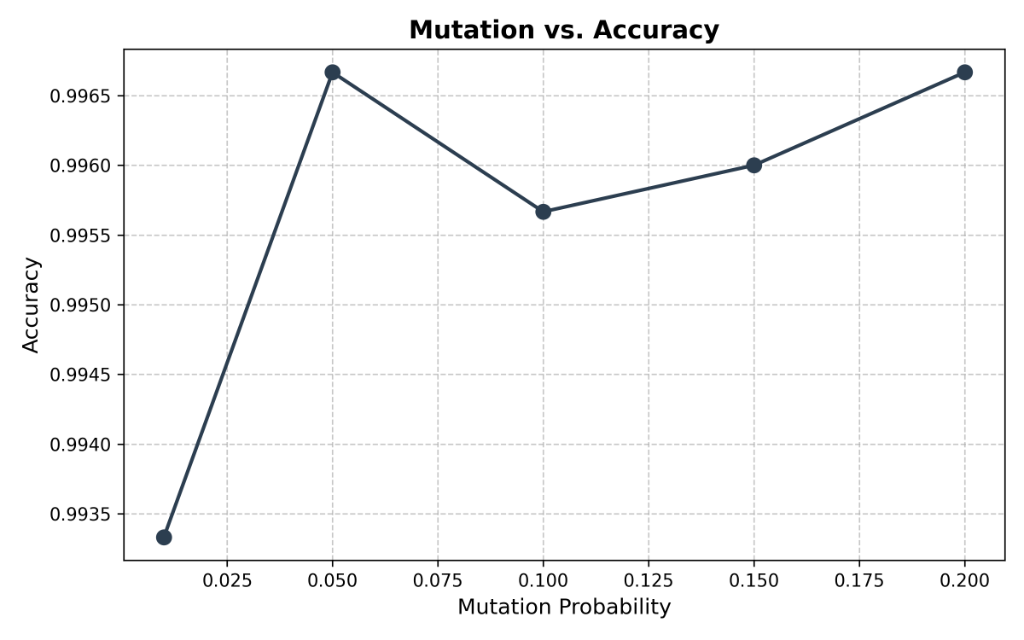
\includegraphics[width=0.48\textwidth]{figures/prof_mut_vs_acc.png}
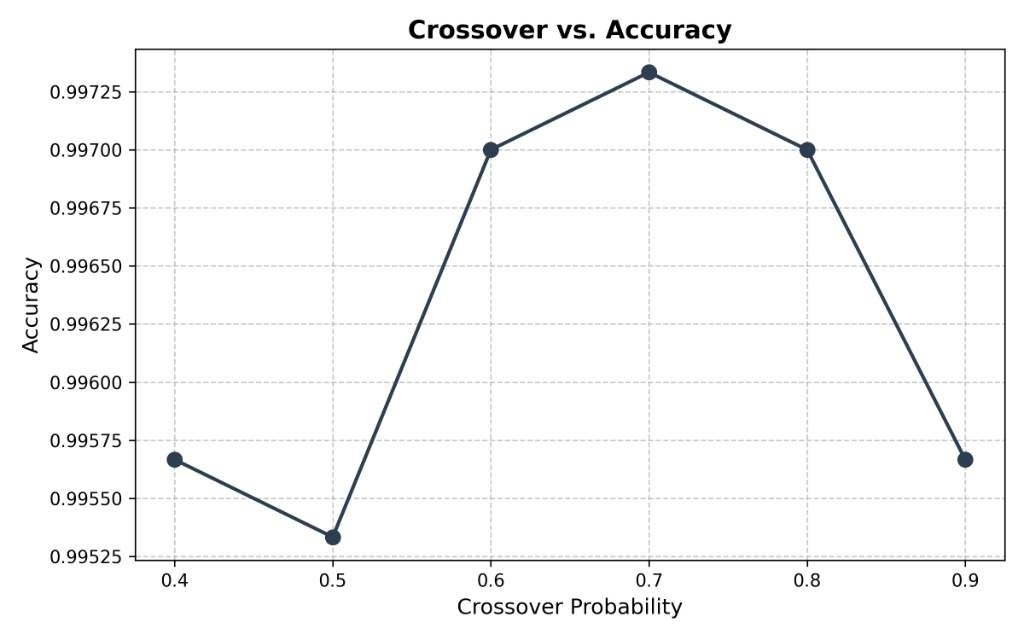
\includegraphics[width=0.48\textwidth]{figures/prof_cx_vs_acc.png}
\caption{Left: Mutation rate vs. Accuracy. Right: Crossover rate vs. Accuracy.}
\end{figure}

\section{ROC Curve and Confusion Matrix}
The performance of the best model (GP3, $\tau=0.9$) is further analyzed using the ROC curve and the confusion matrix across the three lung cancer classes.

\begin{figure}[H]
\centering
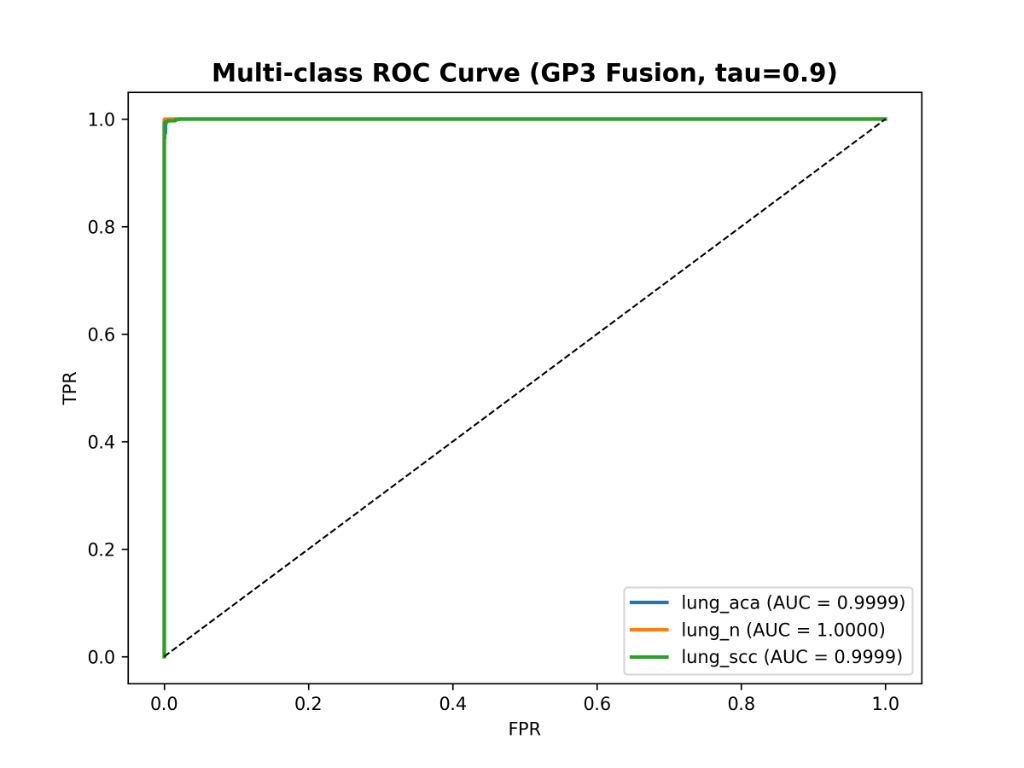
\includegraphics[width=0.7\textwidth]{figures/prof_roc_curve.png}
\caption{Multi-class ROC curve for the proposed method.}
\end{figure}

\begin{figure}[H]
\centering
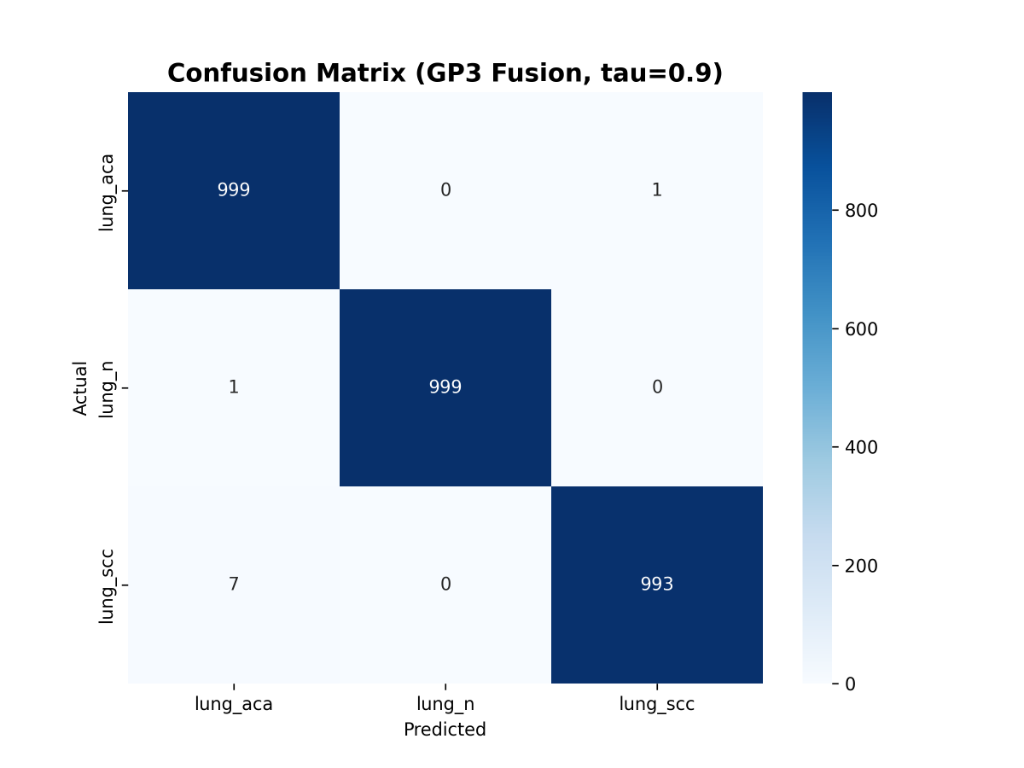
\includegraphics[width=0.7\textwidth]{figures/prof_confusion_matrix.png}
\caption{Confusion matrix for the proposed method.}
\end{figure}

\end{document}
